\chapter{Projektformulering og afgrænsning}
I daglig klinisk praksis er der ofte behov for kontinuert at monitorere patienters blodtryk, i særdeleshed på intensive afdelinger samt operationsstuer, hvor blodtrykket er et vigtigt parameter til monitorering af deres helbredstilstand. \\
Blodtrykket måles invasivt, dvs. at blodtryksmålesystemet er tilsluttet patienternes arterier via et væskefyldt kateter, som afbildet i figuren nedenfor.
\begin{figure}[H]
	\centering
	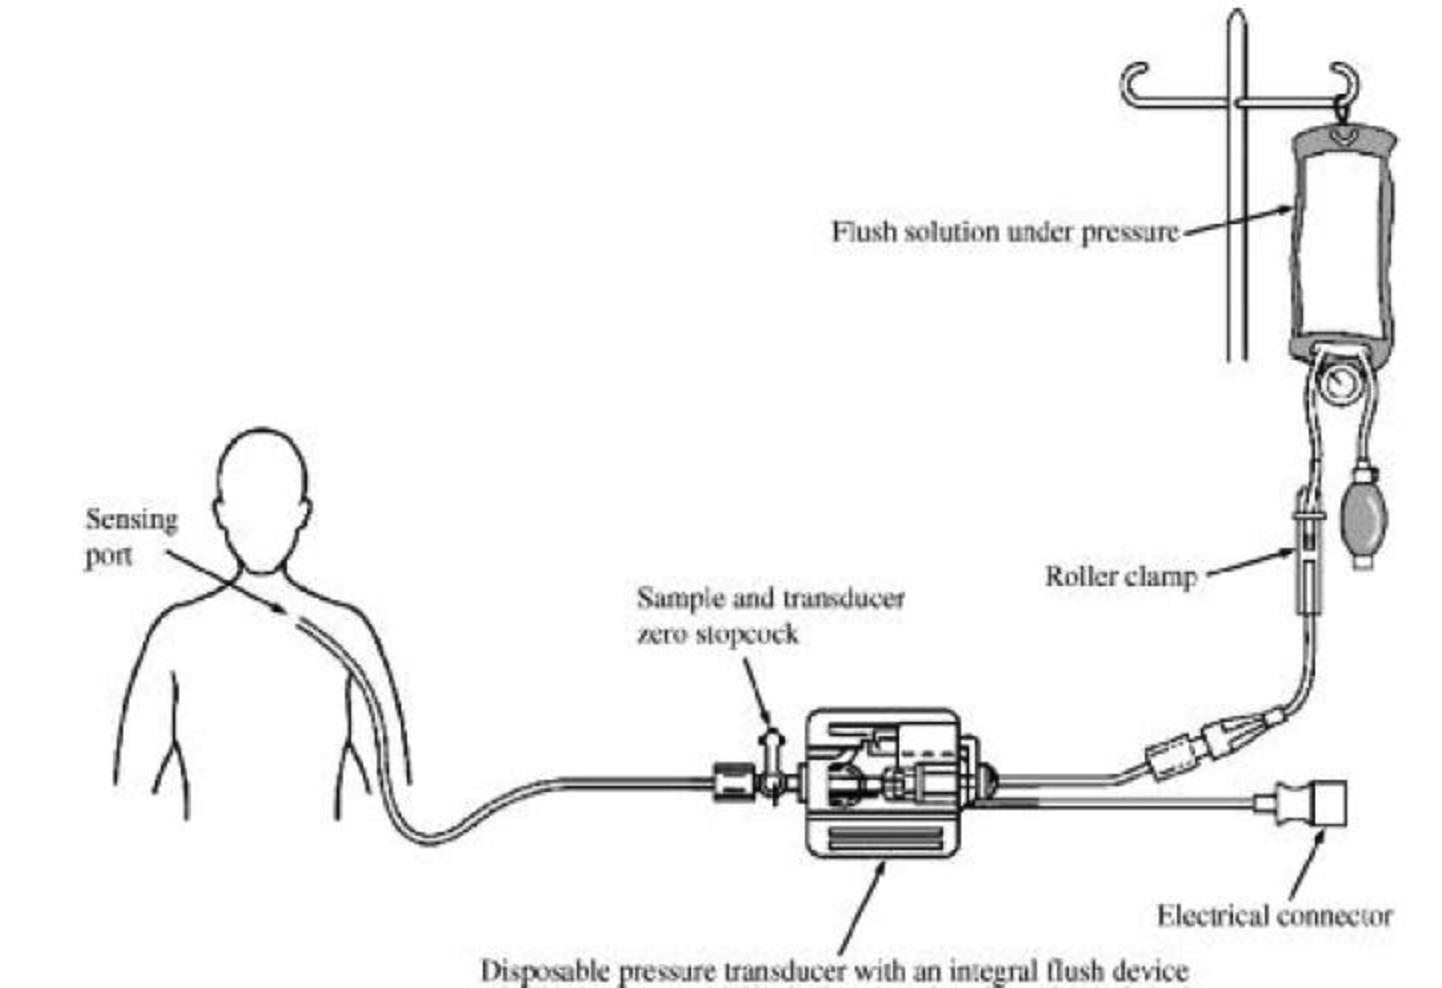
\includegraphics[width=1\textwidth]{Figurer/Snip20151207_50}
	\caption{Måleopstilling, \protect\cite[s. 296]{Billed for invasiv blodtryksmaling}}
\end{figure}

I dette projekt bliver der fokuseret på at udvikle et blodtryksmålersystem, som kan benyttes til forskning, hvor det typisk vil være interessant at observere blodtrykket kontinuerligt. 
Med det in mente, vil der udvikles et blodtryksmålersystem, som kan vise en kontinuerlig blodtrykskurve på en computerskærm.
Systemet realiseres ved udvikling af to elementer, hvoraf det ene består af et elektronisk kredsløb, hvis formål er at forstærke signalet fra tryktransduceren, samt at filtrere signalet med et indbygget analogt filter.\\
Det andet element udmærker sig ved et C\#-program, der skal vise blodtrykket som funktion af tiden. Programmet skal derudover leve op til en række krav for bl.a. kalibrering af blodtrykssignalet, nulpunktsjustering, samt mulighed for at gemme interessante målinger til efterfølgende forskning i en database.
Ydermere er der valgt at afbildede systolisk og diastolisk blodtryk med tal, samt angivelse af pulsværdi.\\\\
Ift. udvikling af vores program har det været nødvendigt, at lave antagelser, hvad angår design af brugergrænsefladen, da der ikke har været kommunikation eller mulighed for test af systemet med slutbrugerne(læger/forskere). 


